\section{Tasklisten}

Die Detailplanung wird auf der Website \href{https://github.com/accefa}{github.com} über ein Issue-System organisiert. Github bietet alle Funktionen, die das Team benötigt und der aktuelle Status des Projektes kann von überall über das Internet abgerufen werden. Es können Meilensteine definiert werden. Diesen Meilensteinen werden Issues (Tasklist) zugewiesen. Innerhalb des Issues definiert man Tasks. Diese Issues können nun den Teammitgliedern zugewiesen werden. Zusätzlich kann man Issues mit Labels kennzeichnen, was den Überblick über das Projekt erheblich erleichtert. Abbildung \ref{fig:github-issue} zeigt die Detailansicht eines Issues. \\ \\
Die kompletten Tasklisten pro Meilenstein sind unter \href{https://github.com/accefa/doku/issues/}{https://github.com/accefa/doku/issues/} abrufbar.

\begin{figure}[!h]
\centering
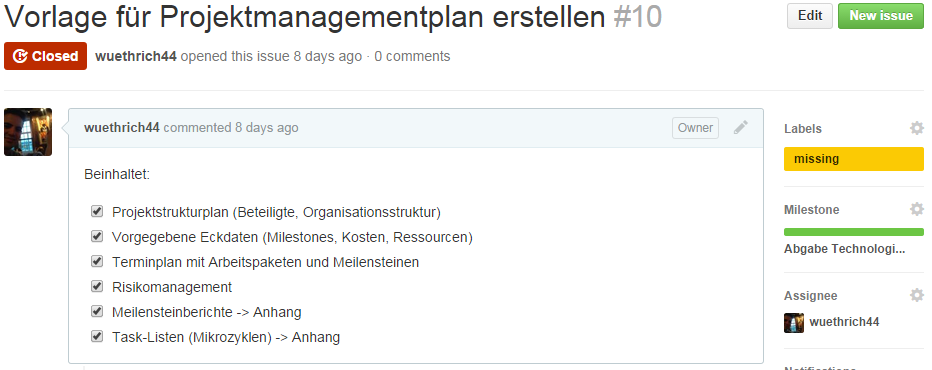
\includegraphics[width=0.7\linewidth]{../../fig/github-issue}
\caption{Github Issue}
\label{fig:github-issue}
\end{figure}
